\documentclass[10pt]{article}
\usepackage[margin=0.62in]{geometry}
\usepackage{graphicx}
\usepackage{booktabs}
\usepackage{hyperref}
\usepackage{parskip}
\hypersetup{colorlinks=true,linkcolor=blue,urlcolor=blue}
\begin{document}
\begin{center}
{\Large\bfseries Semaev first-fall archive replay and trace-witness boundary}\\[3pt]
2026-10-22 --- scoped validation of \texttt{crypto-autoresearcher} main \texttt{4db6ed75}
\end{center}

The original eight-cell toy summary was reproduced byte for byte (SHA-256
\texttt{64f6e34ceb16bd81\ldots 54\,333c99e7}). It records 70 Semaev draws
with first fall at degree two and ten at degree three. The 200 support-matched
null-control draws were also reproduced. No new timing, attack-cost claim,
research-state promotion or performance graph change resulted.

\begin{center}
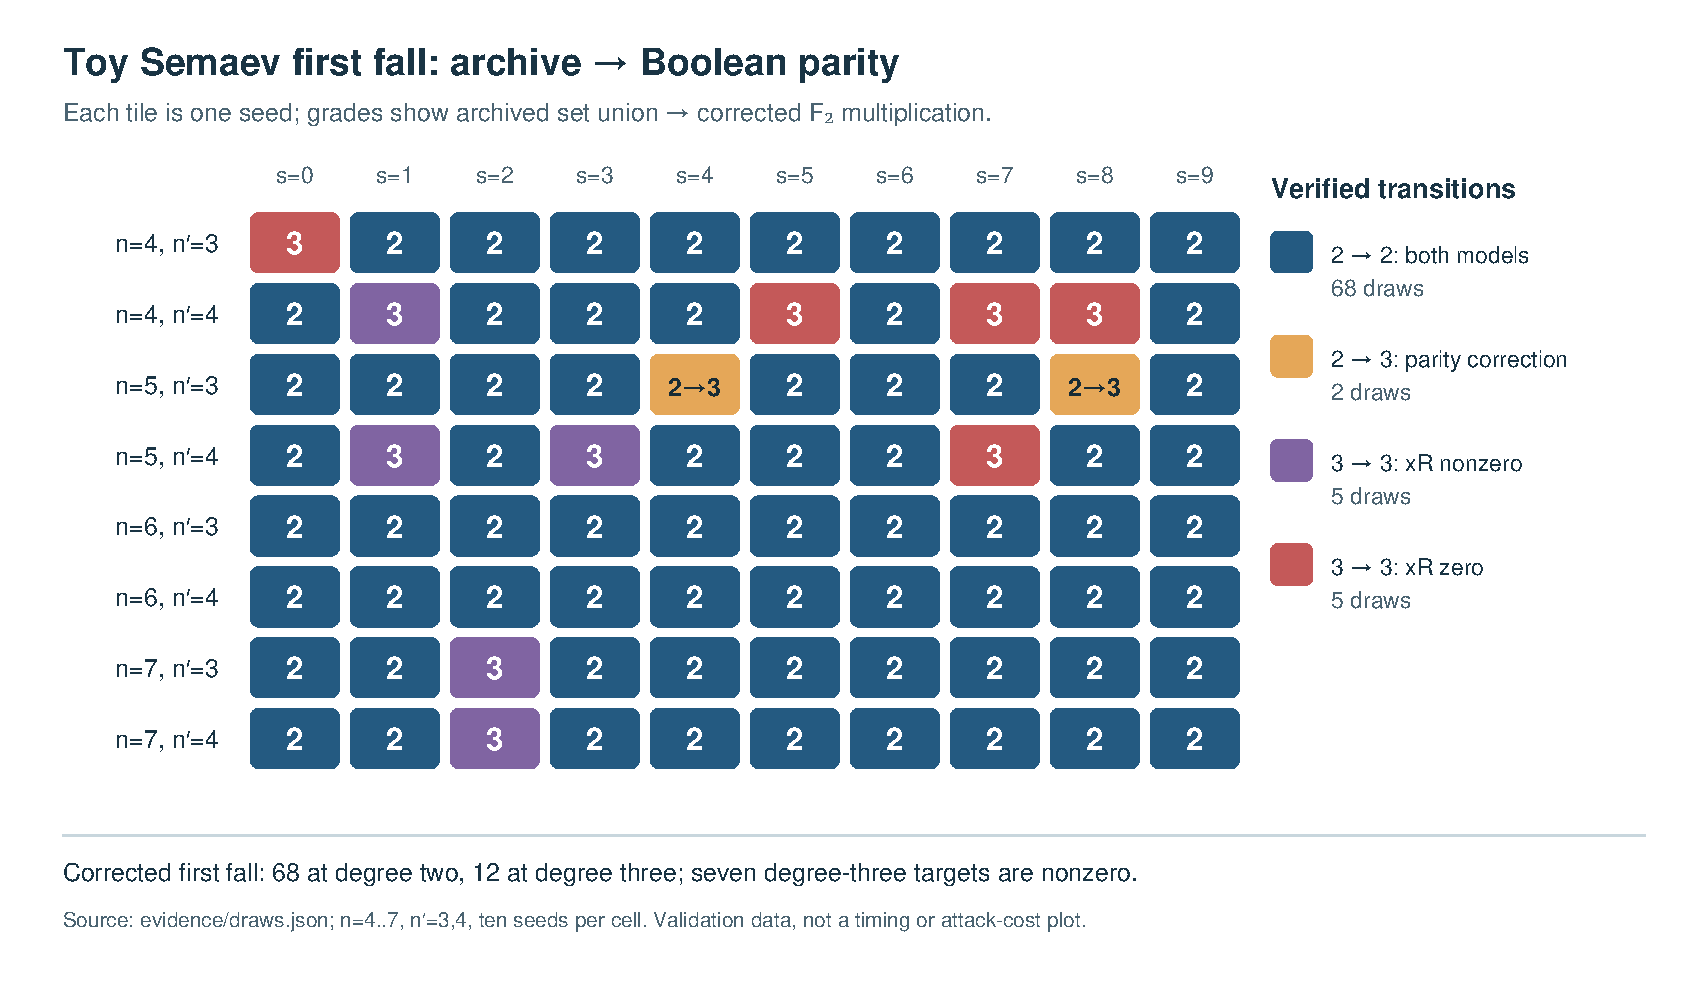
\includegraphics[width=0.9\textwidth]{draws.pdf}
\end{center}
\vspace{-4pt}
\noindent\small Figure: every tile is one archived Semaev seed; the numeral is
the observed first-fall degree. Five degree-three draws have nonzero target
abscissa, so the Lean theorem's $x_R\ne0$ premise alone cannot establish a
uniform degree-two fall. Source: \texttt{evidence/draws.json}; editable renderer:
\texttt{render.py}. This is validation data, not a performance plot.\normalsize

\section*{Independent checks and exact finite example}
The replay checker compared 21,760 finite-field products against an independent
polynomial reduction, evaluated the binary $S_3$ formula on all 12,800 Boolean
assignments in the 80 Semaev draws, and independently recomputed the row-space
rank and degree-projection rank through degree three. It also checked the
support profile and ranks through degree four in all 200 null draws. All
eight Semaev and null distributions match the archived table.

For $n=4$, $n'=4$, seed $s=1$, the target is $x_R=1$ and the factor-base basis
is $[9,3,2,12]$ over the field with modulus $X^4+X+1$. The trace multiplier
is $\mu=x_R^{-2}=1$. Trace cancels the quadratic part, but its nonzero linear
residual $u_0+u_3+w_0+w_3$ is already the fourth input equation. In the
archived Boolean filtration, $\dim V_1=1$ and
$\dim(V_2\cap R_{\le1})=1$, so $\mathrm{new\_falls}(2)=0$.
At degree three, $\dim V_2=11$ and $\dim(V_3\cap R_{\le2})=18$, giving
$\mathrm{new\_falls}(3)=7$. The first fall is therefore three in this
explicit nonzero-target example.

Among all 75 nonzero-target draws, the trace residual is a new class modulo
$V_1$ in 67 degree-two draws. Three other degree-two draws have an old trace
class but a different new relation. Four degree-three draws have a nonzero
trace residual already in $V_1$; one has a zero trace relation. Five additional
degree-three draws have $x_R=0$ and are outside the theorem premise.

\clearpage
\section*{Proof boundary}
The existing \texttt{DegreeTwoFall.lean} proves quadratic trace cancellation,
not the nonzero quotient class required for first fall. This finite example
contradicts a universal degree-two first-fall conclusion for the \emph{archived
Boolean model}; it does not refute the narrower Lean identity or establish a
solving-degree or ECDLP-cost result. A faithful Lean formalization of the
filtration and a checked finite rank counterexample remain open. The frozen
historical target and measurement were not edited. The original 70/10 chart
remains numerically current; this report adds per-draw provenance and trace
classification. Full commands, source hashes, data and limits are in
\texttt{report.md} and \texttt{evidence/}.

\section*{The five nonzero-target exceptions}
\begin{center}
\begin{tabular}{rrrrl}
\toprule
$n$ & $n'$ & seed index $s$ & $x_R$ & Trace residual modulo $V_1$ \\
\midrule
4 & 4 & 1 & 1 & nonzero polynomial, already in $V_1$ \\
5 & 4 & 1 & 19 & nonzero polynomial, already in $V_1$ \\
5 & 4 & 3 & 19 & nonzero polynomial, already in $V_1$ \\
7 & 3 & 2 & 125 & zero polynomial \\
7 & 4 & 2 & 113 & nonzero polynomial, already in $V_1$ \\
\bottomrule
\end{tabular}
\end{center}
\par\medskip
The five remaining degree-three draws have $x_R=0$. Every row above has
$\mathrm{new\_falls}(2)=0$ under the archived definition, independently
recomputed from the Boolean row spaces. Exact bases, equations, residual
monomials and degree-three ranks are in \texttt{evidence/draws.json}.

\section*{Reproduction and remaining work}
The original summary script was run from a scratch directory and its output
compared byte for byte with the committed archive. The source SHA-256 values
for the core, sampler, frozen JSON and independent checker are embedded in
\texttt{evidence/draws.json}. The Python 3.12 checker is
\texttt{replay\_ffd\_semaev\_20261022.py}; its full command and output path are
in \texttt{report.md}. Its field arithmetic and rank routines are
independent of the archived implementations, while the sampler and equation
builder are reused and checked against the direct truth table. The next
formal obligation is to define the archived Boolean filtration in Lean and
prove a finite rank counterexample or a precisely qualified positive theorem.
\end{document}
